%
% Main document
% ===========================================================================
% This is part of the document "Project documentation template".
% Authors: brd3, kaa1
%

%---------------------------------------------------------------------------
\documentclass[
	a4paper,					% paper format
	11pt,							% fontsize
	twoside,					% double-sided
	openright,				% begin new chapter on right side
	notitlepage,			% use no standard title page
	parskip=half,			% set paragraph skip to half of a line
]{scrreprt}					% KOMA-script report
%---------------------------------------------------------------------------

\raggedbottom
\KOMAoptions{cleardoublepage=plain}			% Add header and footer on blank pages


% Load Standard Packages:
%---------------------------------------------------------------------------
\usepackage[standard-baselineskips]{cmbright}

\usepackage[ngerman,english]{babel}										% english hyphenation
%\usepackage[latin1]{inputenc}  							% Unix/Linux - load extended character set (ISO 8859-1)
\usepackage[ansinew]{inputenc}  							% Windows - load extended character set (ISO 8859-1)
\usepackage[T1]{fontenc}											% hyphenation of words with �,� and �
\usepackage{textcomp}													% additional symbols
\usepackage{ae}																% better resolution of Type1-Fonts 
\usepackage{fancyhdr}													% simple manipulation of header and footer 
\usepackage{etoolbox}													% color manipulation of header and footer
\usepackage{graphicx}                      		% integration of images
\usepackage{float}														% floating objects
\usepackage{caption}													% for captions of figures and tables
\usepackage{booktabs}													% package for nicer tables
\usepackage{tocvsec2}													% provides means of controlling the sectional numbering
%---------------------------------------------------------------------------

% Load Math Packages
%---------------------------------------------------------------------------
\usepackage{amsmath}                    	   	% various features to facilitate writing math formulas
\usepackage{amsthm}                       	 	% enhanced version of latex's newtheorem
\usepackage{amsfonts}                      		% set of miscellaneous TeX fonts that augment the standard CM
\usepackage{amssymb}													% mathematical special characters
\usepackage{exscale}													% mathematical size corresponds to textsize
%---------------------------------------------------------------------------

% Package to facilitate placement of boxes at absolute positions
%---------------------------------------------------------------------------
\usepackage[absolute]{textpos}
\setlength{\TPHorizModule}{1mm}
\setlength{\TPVertModule}{1mm}
%---------------------------------------------------------------------------				
\usepackage{booktabs}
\usepackage{multirow}
			
% Definition of Colors
%---------------------------------------------------------------------------
\RequirePackage{color}                          % Color (not xcolor!)
\definecolor{linkblue}{rgb}{0,0,0.8}            % Standard
\definecolor{darkblue}{rgb}{0,0.08,0.45}        % Dark blue
\definecolor{bfhgrey}{rgb}{0.41,0.49,0.57}      % BFH grey
%\definecolor{linkcolor}{rgb}{0,0,0.8}     			% Blue for the web- and cd-version!
\definecolor{linkcolor}{rgb}{0,0,0}        			% Black for the print-version!
%---------------------------------------------------------------------------

% Hyperref Package (Create links in a pdf)
%---------------------------------------------------------------------------
\usepackage[
	pdftex,ngerman,bookmarks,plainpages=false,pdfpagelabels,
	backref = {false},										% No index backreference
	colorlinks = {true},                  % Color links in a PDF
	hypertexnames = {true},               % no failures "same page(i)"
	bookmarksopen = {true},               % opens the bar on the left side
	bookmarksopenlevel = {0},             % depth of opened bookmarks
	pdftitle = {Template f�r Bachelor Thesis},	   	% PDF-property
	pdfauthor = {brd3},        					  % PDF-property
	pdfsubject = {LaTeX Template},        % PDF-property
	linkcolor = {linkcolor},              % Color of Links
	citecolor = {linkcolor},              % Color of Cite-Links
	urlcolor = {linkcolor},               % Color of URLs
]{hyperref}

\usepackage{listings}
\usepackage{color}
\usepackage{amsmath}

\definecolor{dkgreen}{rgb}{0,0.6,0}
\definecolor{gray}{rgb}{0.5,0.5,0.5}
\definecolor{mauve}{rgb}{0.58,0,0.82}

\lstset{frame=tb,
	language=C++,
	aboveskip=3mm,
	belowskip=3mm,
	showstringspaces=false,
	columns=flexible,
	basicstyle={\small\ttfamily},
	numbers=none,
	numberstyle=\tiny\color{gray},
	keywordstyle=\color{blue},
	commentstyle=\color{dkgreen},
	stringstyle=\color{mauve},
	breaklines=true,
	breakatwhitespace=true,
	tabsize=4
}
%---------------------------------------------------------------------------

% Set up page dimension
%---------------------------------------------------------------------------
\usepackage{geometry}
\geometry{
	a4paper,
	left=28mm,
	right=15mm,
	top=30mm,
	headheight=20mm,
	headsep=10mm,
	textheight=242mm,
	footskip=15mm
}
%---------------------------------------------------------------------------

% Makeindex Package
%---------------------------------------------------------------------------
\usepackage{makeidx}                         		% To produce index
\makeindex                                    	% Index-Initialisation
%---------------------------------------------------------------------------

% Glossary Package
%---------------------------------------------------------------------------
% the glossaries package uses makeindex
% if you use TeXnicCenter do the following steps:
%  - Goto "Ausgabeprofile definieren" (ctrl + F7)
%  - Select the profile "LaTeX => PDF"
%  - Add in register "Nachbearbeitung" a new "Postprozessoren" point named Glossar
%  - Select makeindex.exe in the field "Anwendung" ( ..\MiKTeX x.x\miktex\bin\makeindex.exe )
%  - Add this [ -s "%tm.ist" -t "%tm.glg" -o "%tm.gls" "%tm.glo" ] in the field "Argumente"
%
% for futher informations go to http://ewus.de/tipp-1029.html
%---------------------------------------------------------------------------
\usepackage[nonumberlist]{glossaries}
\makeglossaries

\newglossaryentry{BibTeX}{name={BibTeX},description={Program for the creation of 	bibliographical references and directories in \TeX or \LaTeX documents}}
\newglossaryentry{Index}{name={Index},description={Index with keywords from text}}



%---------------------------------------------------------------------------

% Intro:
%---------------------------------------------------------------------------
\begin{document}                              	% Start Document
\settocdepth{section}														% Set depth of toc
\pagenumbering{roman}														
%---------------------------------------------------------------------------

\providecommand{\heading}{Title of Thesis}		%  Insert Title of Thesis here					% Titel der Arbeit aus Datei titel.tex lesen
\providecommand{\versionnumber}{1.0}			%  Hier die aktuelle Versionsnummer eingeben
\providecommand{\versiondate}{06.06.2016}		%  Hier das Datum der aktuellen Version eingeben				% Versionsnummer und -datum aus Datei version.tex lesen

% Set up header and footer
%---------------------------------------------------------------------------
\makeatletter
\patchcmd{\@fancyhead}{\rlap}{\color{bfhgrey}\rlap}{}{}		% new color of header
\patchcmd{\@fancyfoot}{\rlap}{\color{bfhgrey}\rlap}{}{}		% new color of footer
\makeatother

\fancyhf{}																		% clean all fields
\fancypagestyle{plain}{												% new definition of plain style	
	\fancyfoot[OR,EL]{\footnotesize \thepage} 	% footer right part --> page number
	\fancyfoot[OL,ER]{\footnotesize \heading, Version \versionnumber, \versiondate}	% footer even page left part 
}

\renewcommand{\chaptermark}[1]{\markboth{\thechapter.  #1}{}}
\renewcommand{\headrulewidth}{0pt}				% no header stripline
\renewcommand{\footrulewidth}{0pt} 				% no bottom stripline

\pagestyle{plain}
%---------------------------------------------------------------------------


% Title Page and Abstract
%---------------------------------------------------------------------------
%%
% Project documentation template
% ===========================================================================
% This is part of the document "Project documentation template".
% Authors: brd3, kaa1
%

\begin{titlepage}


% BFH-Logo absolute placed at (28,12) on A4 and picture (16:9 or 15cm x 8.5cm)
% Actually not a realy satisfactory solution but working.
%---------------------------------------------------------------------------
\setlength{\unitlength}{1mm}
\begin{textblock}{20}[0,0](28,12)
	
\includegraphics[scale=1.0]{images/BFH_Logo_B.png}
\end{textblock}

% Institution / titel / subtitel / authors / experts:
%---------------------------------------------------------------------------
\begin{flushleft}

\vspace*{21mm}

\fontsize{26pt}{40pt}\selectfont 
\heading				\\							% Read heading from file leader/title.tex
\vspace{2mm}

\fontsize{16pt}{24pt}\selectfont\vspace{0.3em}
Place your subheading here 			\\				% Insert subheading
\vspace{5mm}

\fontsize{10pt}{12pt}\selectfont
\textbf{Description of thesis (semester- / Bachelor thesis / etc.)} \\		% Insert text
\vspace{7mm}

% Abstract (eingeben):
%---------------------------------------------------------------------------
\begin{textblock}{150}(28,100)
\fontsize{10pt}{12pt}\selectfont
[Insert short text (abstract) if desired] \\ 
This document serves as a template for the compilation of reports according to the guidelines of the BFH. The template is written in LATEX and supports the automatic writing of various directories, references, indexing and glossaries. This small text is a summary of this document with a length of 4 to max. 8 lines. \\ 
The cover picture may be turned on or off in the lines 157/158 of the file template.tex.
\end{textblock}

\begin{textblock}{150}(28,225)
\fontsize{10pt}{17pt}\selectfont
\begin{tabbing}
xxxxxxxxxxxxxxx\=xxxxxxxxxxxxxxxxxxxxxxxxxxxxxxxxxxxxxxxxxxxxxxx \kill
Degree course:	\> [z.B. Electrical and Communication Engineering]	\\		% insert name of degree course
Authors:		\> [Test Peter, M\"uster R\"os\"a]		\\					% insert names
Tutor:	\> [Dr.~Xxxx Xxxx, Dr.~Yyyy Yyyy]		\\							% insert names
Constituent:	\> [Wwwww AG]					\\							% insert names
Experts:		\> [Dr.~Zzzz Zzzz]				\\							% insert names
Date:			\> \versiondate					\\							% read from file leader/version.tex
\end{tabbing}

\end{textblock}
\end{flushleft}

\begin{textblock}{150}(28,280)
\noindent 
\color{bfhgrey}\fontsize{9pt}{10pt}\selectfont
Berner Fachhochschule | Haute \'ecole sp\'ecialis\'ee bernoise | Bern University of Applied Sciences
\color{black}\selectfont
\end{textblock}


\end{titlepage}

%
% ===========================================================================
% EOF
%
		% activate for frontpage without picture
%
% Project documentation template
% ===========================================================================
% This is part of the document "Project documentation template".
% Authors: brd3, kaa1
%

\begin{titlepage}


% BFH-Logo absolute placed at (28,12) on A4 and picture (16:9 or 15cm x 8.5cm)
% Actually not a realy satisfactory solution but working.
%---------------------------------------------------------------------------
\setlength{\unitlength}{1mm}
\begin{textblock}{20}[0,0](28,12)
	
\includegraphics[scale=1.0]{images/BFH_Logo_B.png}
\end{textblock}

\begin{textblock}{154}(28,48)
	\begin{picture}(150,2)
		\put(0,0){\color{bfhgrey}\rule{150mm}{2mm}}
	\end{picture}
\end{textblock}

\begin{textblock}{154}[0,0](28,50)
	
\includegraphics[scale=1.0]{images/placemarker.jpg}			% define cover picture
\end{textblock}

\begin{textblock}{154}(28,135)
	\begin{picture}(150,2)
		\put(0,0){\color{bfhgrey}\rule{150mm}{2mm}}
	\end{picture}
\end{textblock}
\color{black}

% Institution / titel / subtitel / authors / experts:
%---------------------------------------------------------------------------
\begin{flushleft}

\vspace*{115mm}

\fontsize{26pt}{28pt}\selectfont 
\heading				\\							% Read heading from file leader/title.tex
\vspace{2mm}

\fontsize{16pt}{20pt}\selectfont\vspace{0.3em}
Place your subheading here 			\\				% Insert subheading
\vspace{5mm}

\fontsize{10pt}{12pt}\selectfont
\textbf{Description of thesis (semester- / Bachelor thesis / etc.)} \\		% Insert text
\vspace{3mm}

% Abstract (eingeben):
%---------------------------------------------------------------------------
\begin{textblock}{150}(28,190)
\fontsize{10pt}{12pt}\selectfont
[Insert short text (abstract) if desired] \\ 
This document serves as a template for the compilation of reports according to the guidelines of the BFH. The template is written in LATEX and supports the automatic writing of various directories, references, indexing and glossaries. This small text is a summary of this document with a length of 4 to max. 8 lines. \\ 
The cover picture may be turned on or off in the lines 157/158 of the file template.tex.
\end{textblock}

\begin{textblock}{150}(28,225)
\fontsize{10pt}{17pt}\selectfont
\begin{tabbing}
xxxxxxxxxxxxxxx\=xxxxxxxxxxxxxxxxxxxxxxxxxxxxxxxxxxxxxxxxxxxxxxx \kill
Degree course:	\> [z.B. Electrical and Communication Engineering]	\\		% insert name of degree course
Authors:		\> [Test Peter, M\"uster R\"os\"a]		\\					% insert names
Tutor:	\> [Dr.~Xxxx Xxxx, Dr.~Yyyy Yyyy]		\\							% insert names
Constituent:	\> [Wwwww AG]					\\							% insert names
Experts:		\> [Dr.~Zzzz Zzzz]				\\							% insert names
Date:			\> \versiondate					\\							% read from file leader/version.tex
\end{tabbing}

\end{textblock}
\end{flushleft}

\begin{textblock}{150}(28,280)
\noindent 
\color{bfhgrey}\fontsize{9pt}{10pt}\selectfont
Berner Fachhochschule | Haute \'ecole sp\'ecialis\'ee bernoise | Bern University of Applied Sciences
\color{black}\selectfont
\end{textblock}


\end{titlepage}

%
% ===========================================================================
% EOF
%
		% activate for frontpage with picture
% Control of versions :
% -----------------------------------------------

\begin{textblock}{180}(15,150)
\color{black}
\begin{huge}
Versions
\end{huge}
\vspace{10mm}

\fontsize{10pt}{18pt}\selectfont
\begin{tabbing}
xxxxxxxxxxx\=xxxxxxxxxxxxxxx\=xxxxxxxxxxxxxx\=xxxxxxxxxxxxxxxxxxxxxxxxxxxxxxxxxxxxxxxxxxxxxxx \kill
Version	\> Date	\> Status			\> Remarks		\\
0.1	\> 16.05.2016	\> Draft		\> Create Document	\\	
0.2	\> 06.06.2016	\> Draft		\> First Complete Draft	\\ 	
\end{tabbing}

\end{textblock}

\cleardoubleemptypage
\setcounter{page}{1}
\cleardoublepage
\phantomsection 
\addcontentsline{toc}{chapter}{Management Summary}
\chapter*{Management Summary}
\label{chap:managementSummary}

Eye tracing has a wide area of applications such as sports and psychology. To analyze gaze direction from a eye-tracking system for sports, software is needed that can display the gaze position on a video playback. Each gaze point needs to be synchronized with the video. 

The target for this project was to develop such a software that can be expanded later but is feature complete so that it can be used for analyzing footage and gaze data.

\cleardoubleemptypage
%---------------------------------------------------------------------------

% Table of contents
%---------------------------------------------------------------------------
\tableofcontents
\cleardoublepage
%---------------------------------------------------------------------------

% Main part:
%---------------------------------------------------------------------------
\pagenumbering{arabic}

\chapter{Introduction}
\label{chap:introduction}



% Eintr�ge im Verzeichnis erscheinen lassen ohne hier eine Referenz einzuf�gen
\nocite{kopka:band1}
\nocite{raichle:bibtex_programmierung}
\nocite{MiKTeX}
\nocite{KOMA}
\nocite{TeXnicCenter}
\nocite{Marti06}
\nocite{Erbsland08}
\nocite{juergens:einfuehrung}
\nocite{juergens:fortgeschritten}

\section{Organising Documents}
\label{sec:einleitung_aufbau}
Eye tracking is used to measure where someone is looking. It is used in a wide variety of applications such as marketing research, psychology, virtual reality and sports training. 

To enable high speed eye tracking for sports the HuCE developed an eye tracking system called the Gazelle Eye Tracker that is fast, portable and built for outdoor usage. The  

For analyzing the recorded footage a player that can put an overlay over the video playback.



\section{Requirements}
\label{sec:introduction_contact}

There a few key requirements that can be categorized in optional and must have. This is done in \ref{tab:requirements}. 

\begin{table}[H]
	\centering
	\begin{tabular}{lcc} \toprule
		\textbf{Requirement} & \textbf{must} & \textbf{optional} \\ \midrule
		Play video & x &  \\ \midrule
		Video has overlay & x &  \\ \midrule
		Step frame for frame \\ forward and backward& x &  \\ \midrule
		Step overlay for overlay \\ forward and backward& x &  \\ \midrule
		Overlay and Frames are in sync & x &  \\ \midrule
		Display data of eye-cameras &  & x \\ \midrule
		Play at various playspeeds &  & x \\ \midrule
		Play overlays &  & x \\ \midrule
	\end{tabular}
	\caption{List of requirements }
	\label{tab:requirements}
\end{table}


\chapter{Gazelle View}
\label{chap:gazelleView}
 Gazelle View is the software developed in this project. 
 \begin{figure}[H]
 	\centering
 	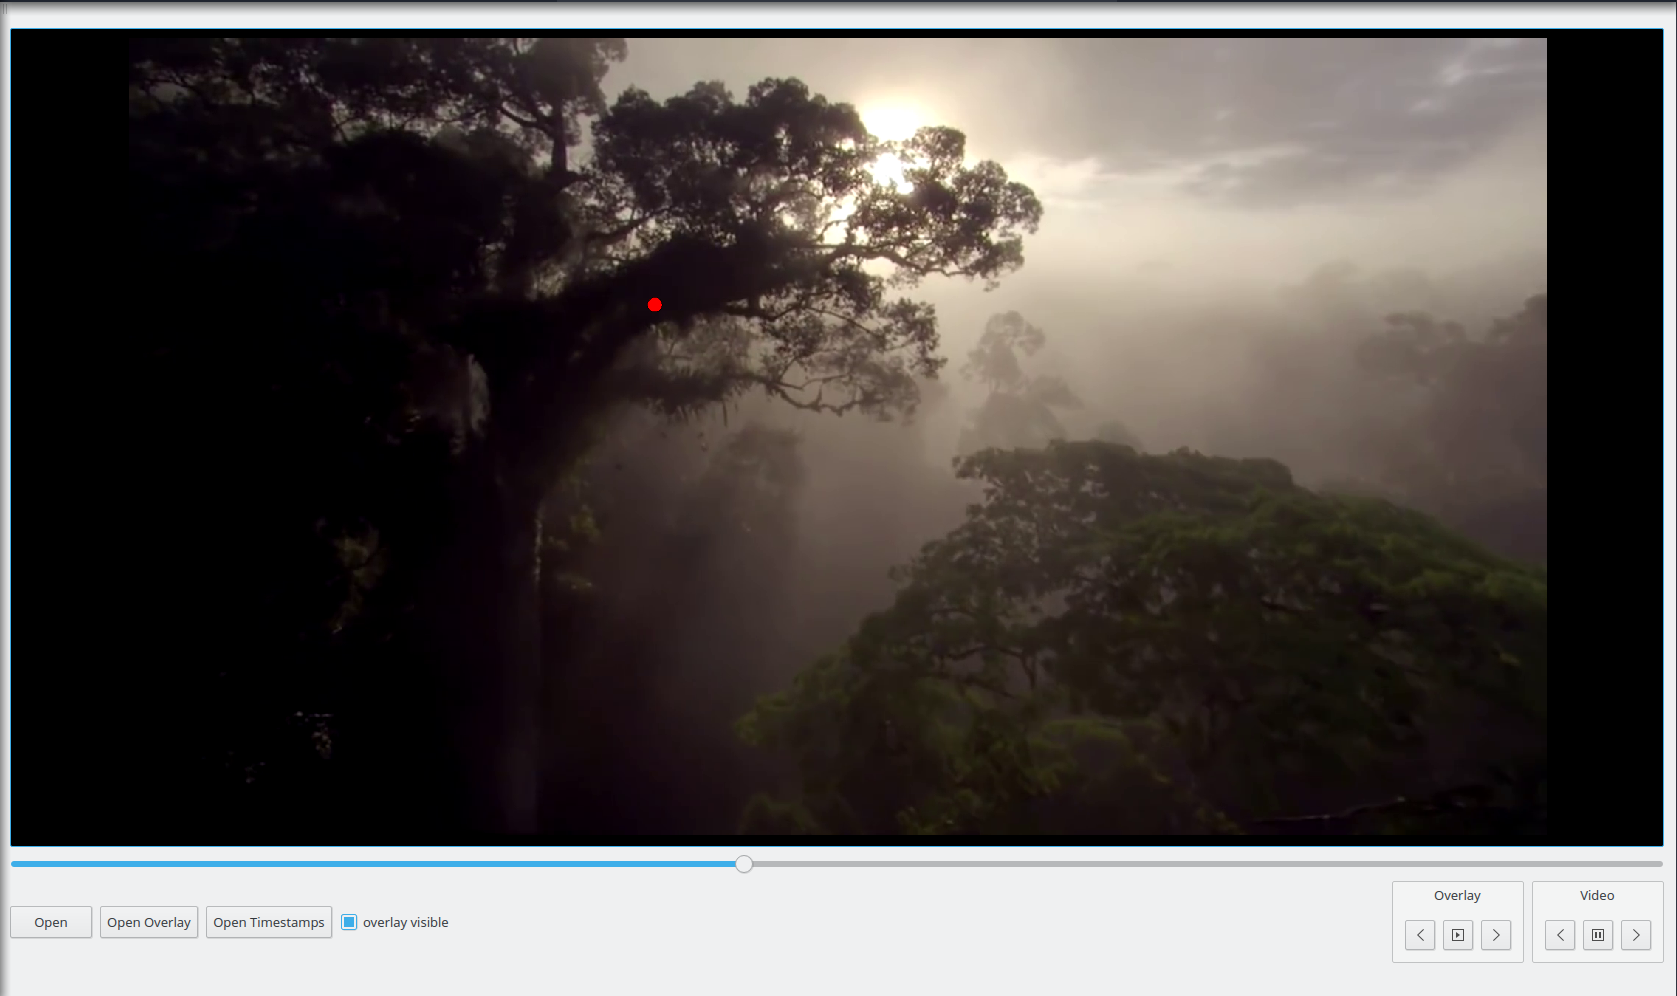
\includegraphics[scale=0.25]{images/gui_gazelle_view.png}
 	\caption{GUI of Gazelle View with the Breeze icon theme}
 	\label{fig:guiGazelleView}
 \end{figure}
\section{Use cases}
\label{sec:useCases}
The use cases for Gazelle View are presented in \ref{fig:useCases} and are deducted from the requirements.
\begin{itemize}
	\item The user can open a video, overlays and timestamps
	\item The user can play the video
	\item The user can pause the video
	\item The user can go to the next or previous frame
	\item The user can play overlays
	\item The user can pause overlays
	\item The user can go to the next or previous overlay
\end{itemize}
\section{Class Diagram}
Gazelle View is build with four classes as seen in \ref{fig:classDIagram} The GUI is handled by the class MainWindow. User input is forwarded to the class VideoHandler. VideoHandler is in control of which overlay and frame are displayed or decoded and it also manages the buffer. Because decoding is an expensive operation, so VideoHandler orders frames to be decoded from DecodeWorker. DecodeWorker has as sole instance access to the videostream and has to provide metadata such as framerate and how total count of frames in the stream. DecodeWorker runs in it's own thread so it doesn't block the other classes. The class Overlays is responsible to parse overlays and timestamps and find the corresponding frame or overlay for a timestamp.
\subsection{MainWindow}
\label{sec:mainWindow}
MainWindow handles the GUI, user input and displays the image with the overlay. It extends from QMainWindow and allows using the signal/slot framework from Qt. 
MainWindow sets up the icons of the play/pause, back and forwards buttons for overlay and video so that they use the icon theme of the current desktop environment. Fallback icons are provided for system that don't have themes or themes that don't have the necessary icons. An example of the GUI with the Breeze icon theme from KDE can be seen in \ref{fig:guiGazelleView}.

The communication with the class VideoHandler is done over the signal/slot framework from qt. The slot "displayImage" gets called when VideoHandler want's to display a new image. This image is shown on a QGraphicsScene with black background.
\subsection{VideoHandler}
\label{sec:videoHanlder}
VideoHandler handles a few things.
\begin{itemize}
	\item Order new frames to be decoded
	\item Send a frame to be displayed
	\item Handle the framebuffer
	\item Keep overlays and Frames in sync
	\item Send overlays to be displayed
\end{itemize}
VideoHandler extends QObject to communicate with the other classes over the signal/slot framework.

VideoHandler relies on DecodeWorker to decode the frames in a separate thread and on Overlays for getting the information which overlay needs to be displayed on which frame.
\subsubsection{Framebuffer}
\label{sec:framebuffer}
As decided in \ref{sec:frameBuffer} this is done with a QHash with the framenumber as key and a pointer to the Image as value. The buffer is trailing so it stores the last 50-100 frames. This is because the stream can only be decoded forward and jumping to a previous frame is expensive. To keep the size of the framebuffer reasonable a method iterates over the QHash when it get's to large and deletes all frames that are more than 50 frames behind.
\subsection{Overlay}
\label{sec:overlayClass}
The class Overlays is responsible for the following things.
\begin{itemize}
	\item parse file with information about overlays
	\item parse file of timestamps for the frames
	\item store overlays and timestamps
	\item return the overlay before or after a timestamp
	\item return the frame before a timestamp
	\item return the timestamp for a certain frame
\end{itemize}
The unit of the timestamps don't matter as long as they are the same for overlays and frames. 
As discussed in \ref{sec:overlays} a QMap stores the information for the overlays. The next or previous overlay is accessible for a timestamp. Additionally the corresponding timestamp for the overlay is also returned.
\subsubsection{Timestamps for Frames}
\label{sec:timestampsForFrames}
It is required to provide access for both the timestamp for a certain frame and the frame for a certain timestamp. In \ref{sec:timestamps} successive approximation was proposed to solve this issue. The implementation is as follows:

\begin{lstlisting}
for (int i = size/2; i >= 1; i /= 2) {
	if ((frameCount > (currentFrame + i)) &&
		    (_sceneFrames.at(currentFrame + i) < timestamp)) {
		currentFrame += i;
	}
}
\end{lstlisting}
\begin{itemize}
	\item \texttt{\_sceneFrames} is the QVector that stores timestamps
	\item \texttt{frameCount} is the size of \texttt{\_sceneFrames}
	\item \texttt{size} is the next higher power of two after \texttt{frameCount}
	\item \texttt{currentFrame} holds the result at the end of the algorithm
	\item \texttt{currentFrame +  i} is the frameindex that is tested
\end{itemize}
The result converges to the frameindex that has the timestamp below the timestamp that is supplied. It does so by comparing the supplied timestamp with the timestamp at index $\displaystyle\frac{\mbox{\texttt{size}}}{\mbox{2}}$ of \texttt{\_sceneFrames} first and followed by either $\displaystyle\frac{\mbox{\texttt{size}}}{\mbox{4}}$ or $\displaystyle\frac{\mbox{3 x \texttt{size}}}{\mbox{4}}$ depending on the outcome of the comparison. This goes on until the increment is one.

\subsection{DecodeWorker}
\label{sec:decodeWorker}
The job of the DecodeWorker is to decode frames and convert them into a usable format so that the frame can be displayed on screen on a QGraphicScene. A library that enables decoding frames and give access to the pixeldata of each frame is OpenCV. It would also be possible to play videos with QMultiMedia. The disadvantage of this is that there is no direct access to each frame and the pixel data. OpenCV was chosen because i in the future it might be a requirement to manipulate or analyze each frame of the stream and OpenCV provides many tools that enable that.

Decoding and converting a video stream takes time so DecodeWorker is moved to it's own thread so it doesn't block the GUI or other parts of the program. Resulting race conditions are mitigated by the use of QMutex.

\subsubsection{Getting a Frame Ready}
\label{sec:gettingAFrameReady}
The frame needs to be stored as a QPixMapItem in order to be displayed on a QGraphicsScene. This is done by a few steps:
\begin{enumerate}
	\item Decode a single frame with OpenCV into a Mat
	\item Convert the Mat from BGR to RGB
	\item Transfer the picture data from the Mat to a QImage
	\item convert the QImage to a QPixMap
\end{enumerate}

The second step is required because OpenCV stores its images in the BGR format instead of the more common RGB format.

%The index doubles every iteration and the target timestamp is compared with the %timestamp at the frameindex of the current iteration. Access to  to non-existent %entries are prevented by comparing the frameindex to the size of %\texttt{\_sceneFrames}. The resulting frameindex is set to the tested frameindex %when the timestamp at said index is smaller than the reference timestamp. Otherwise %\texttt{currentFrame} stays the same. 

\section{Glossay}
\label{sec:instructions_glossay}

A glossary\index{glossary} can also be created in \LaTeX{} with the \texttt{makeindex} program and the \texttt{glossaries} package. The following list shows the procedure to generate a glossary:

\begin{itemize}
	\item Integration of the package \texttt{glossaries}.
	\item If necessary, a personal database may be created including glossary entries. This template works with such a database, which is stored in the \texttt{database}folder. Entries from the database are only written in the directory if the word in the text is actually stated.
	\item With the \texttt{\textbackslash makeglossaries} command a new compilation is initialized.
	\item New entries can be created with the command \\ \texttt{\textbackslash newglossaryentry\{<SHORTCUT>\}\{name=\{<NAME>\},description=\{<DESCRIPTION>\}\}}.
	\item In the text continuously referencing words with the command \texttt{\textbackslash gls\{<SHORTCUT>\}}.
	\item Similar to the compilation of the index, the directory is only embedded into the document  during the second passage.
\end{itemize}

In order to work accurately, the glossary must be compiled with \texttt{makeindex} after post-editing the document. For this the following code in the command line is to be executed:

\begin{center}
	\texttt{makeindex -s template.ist -t template.glg -o template.gls template.glo}
\end{center}

With most \LaTeX editors, this can be stated as a post-processing step. The following explanation is for the TeXnicCenter program. Under the menu "Build" > "Define Output Profile..." (short: alt + F7) in the "Postprocessor" register, the window shown in Figure \ref{fig:postprocessing} can be found. Then it is necessary to insert a new entry, when an application as well as an argument must be specified. The application can be found in the MiKTeX installation (\texttt{..\textbackslash MiKTeX X.X\textbackslash miktex\textbackslash bin\textbackslash makeindex.exe}). As an argument, the following line must be entered:

\begin{center}
	\texttt{-s \string"\%tm.ist\string" -t \string"\%tm.glg\string" -o \string"\%tm.gls\string" \string"\%tm.glo\string" }
\end{center}

\begin{figure}[H]
	\centering
		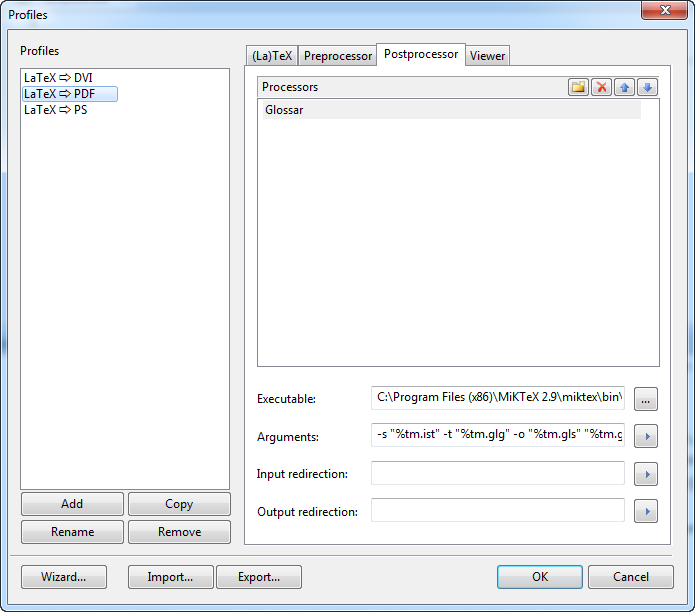
\includegraphics[scale=0.6]{images/profiles_glossar.png}
	\caption{Post-processing}
	\label{fig:postprocessing}
\end{figure}


\section{Bibliography}
\label{sec:instructions_bibliography}

To compile a bibliography\index{bibliography} one must resort to \gls{BibTeX}. The folder \texttt{database} includes a \texttt{.bib} file with various database entries. How the entries are to be compiled, can be taken from various sources of the Internet or books. The entries in the database will only be written to the directory of the document when the source is actually cited in the text.

Under the following addresses further explanations are found in order to compile the database and its use:

\begin{itemize}
	\item \url{http://en.wikipedia.org/wiki/BibTeX}
	\item \url{http://www.bibtex.org/}
\end{itemize}



\chapter{Software Design}
\label{chap:typeareatest}

Far far away, behind the word mountains, far from the countries Vokalia and Consonantia, there live the blind texts. Separated they live in Bookmarksgrove right at the coast of the Semantics, a large language ocean. A small river named Duden flows by their place and supplies it with the necessary regelialia. It is a paradisematic country, in which roasted parts of sentences fly into your mouth. Even the all-powerful Pointing has no control about the blind texts it is an almost unorthographic life One day however a small line of blind text by the name of Lorem Ipsum decided to leave for the far World of Grammar. 

\section{Software Architecture}
\label{sec:typeareatest_ombox}

The Big Oxmox advised her not to do so, because there were thousands of bad Commas, wild Question Marks and devious Semikoli, but the Little Blind Text didn’t listen. She packed her seven versalia, put her initial into the belt and made herself on the way. When she reached the first hills of the Italic Mountains, she had a last view back on the skyline of her hometown Bookmarksgrove, the headline of Alphabet Village and the subline of her own road, the Line Lane. Pityful a rethoric question ran over her cheek, then she continued her way. On her way she met a copy.

\begin{equation}
	\mathcal{N}(x \mid \mathbold{\mu}, \mathbold{\Sigma}) = \frac{1}{(2\pi)^{D/2}} \frac{1}{|\mathbold{\Sigma}|^{(1/2)}} \exp \left( -\frac{1}{2}(x-\mathbold{\mu})^{T}\mathbold{\Sigma}^{-1}(x-\mathbold{\mu}) \right)
\end{equation}

The copy warned the Little Blind Text, that where it came from it would have been rewritten a thousand times and everything that was left from its origin would be the word "and" and the Little Blind Text should turn around and return to its own, safe country. But nothing the copy said could convince her and so it didn’t take long until a few insidious Copy Writers ambushed her, made her drunk with Longe and Parole and dragged her into their agency, where they abused her for their projects again and again. And if she hasn’t been rewritten, then they are still using her.

\section{Design Decisions}
\label{sec:typeareatest_typedummytext}

This is a typo dummy text. On it you can see if all the letters there are and how they look. Sometimes one uses words like Hamburgefonts, Rafgenduks or Handgloves to test fonts. Sometimes phrases that contain all letters of the alphabet - one calls these sets "pangrams".

Well known is this: The quick brown fox jumps over the lazy old dog. Often in type dummy texts also foreign-language sentence parts are installed (AVAIL\textsuperscript{\texttrademark} and Wefox\textsuperscript{\textregistered} are testing aussi la Kerning) to test the effect in other languages. In Latin, for example, almost every font looks good.

\subsection{Storage Containers}
\label{subsec:satzspiegeltest_typoblindtext_demonstrandum}

Qt has an implementations for all popular storage containers. They all have different structures and are intended for different applications. The Containers can be categorized in two major categories. The first is index lookup where each element is stored at a certain index. The second is key lookup and all elements are stored with a key.

% Please add the following required packages to your document preamble:
% \usepackage{booktabs}
% \usepackage{multirow}
\begin{table}[]
\centering

\label{my-label}
\begin{tabular}{@{}|l|l|l|l|l|@{}}
\toprule
\multirow{2}{*}{}                    & \multicolumn{2}{l|}{Key lookup} & \multicolumn{2}{l|}{Insertion} \\ \cmidrule(l){2-5} 
                                     & Average         & Worst Case    & Average        & Worst case    \\ \midrule
QMap\textless Key, T\textgreater      & O(log n)        & O(log n)      & O(log n)       & O(log n)      \\ \midrule
QMultiMap\textless Key, T\textgreater & O(log n)        & O(log n)      & O(log n)       & O(log n)      \\ \midrule
QHash\textless Key, T\textgreater     & Amort. O(1)     & O(n)          & Amort. O(1)    & O(n)          \\ \midrule
QSet\textless Key\textgreater     & Amort. O(1)     & O(n)          & Amort. O(1)    & O(n)          \\ \bottomrule
\end{tabular}
\caption{Algorithmic Complexity of Qt-Container with key lookup and insertion
\end{table}

\subsubsection{Subsubsection}

This is a typo dummy text. On it you can see if all the letters there are and how they look. Sometimes one uses words like Hamburgefonts, Rafgenduks or Handgloves to test fonts. Sometimes phrases that contain all letters of the alphabet - one calls these sets "pangrams". 

\subsubsection{Subsubsection}

Well known is this: The quick brown fox jumps over the lazy old dog. Often in type dummy texts also foreign-language sentence parts are installed (AVAIL\textsuperscript{\texttrademark} and Wefox\textsuperscript{\textregistered} are testing aussi la Kerning) to test the effect in other languages. In Latin, for example, almost every font looks good. Quod erat demonstrandum.

\section{Webstandards}
\label{sec:satzspiegeltest_webstandards}

Everywhere the same old story. The layout is complete, the text is slow in coming. This layout is now not naked in space and small and empty occurs, I help out: the dummy text. Created exactly for this purpose, always in the shadow of my big brother "Lorem Ipsum", I look forward every time you read a few lines. Because esse est percipi - being is to be perceived.

And now because you already have the goodness to accompany me a few more sentences long, I would like to take this opportunity to serve you not only as a stopgap, but to point out something that is going to be perceived as deserved: Web viz. See Web standards are the rules that build on the websites. So there are rules for HTML, CSS, JavaScript or XML, words that you might have heard of your developers. These standards ensure that all parties the maximum benefit from a website.

\begin{figure}[H]
	\centering
		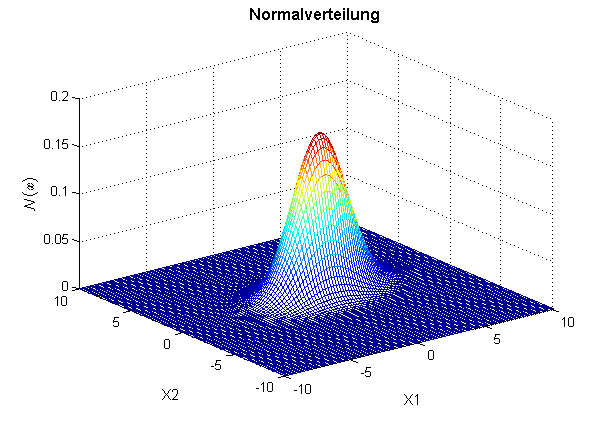
\includegraphics[scale=0.7]{images/multivariate_gauss.png}
	\caption{Normal distribution}
	\label{fig:normal_distribution}
\end{figure}

In contrast to previous websites we no longer need, for example, two different sites for the program Internet Explorer and another browser. It extends a page that - properly applied - both works on different browsers on the net, but just as good for printing or display on a cell phone is. Mind: A site for all formats. What a relief. Standards save time provide for the development costs and ensure that web pages can be easier to maintain later. Of course, only if everyone adheres to these standards.

\chapter{Conclusion / Results}
\label{chap:conclusions}

But I must explain to you how all this mistaken idea of denouncing pleasure and praising pain was born and I will give you a complete account of the system, and expound the actual teachings of the great explorer of the truth, the master-builder of human happiness. No one rejects, dislikes, or avoids pleasure itself, because it is pleasure, but because those who do not know how to pursue pleasure rationally encounter consequences that are extremely painful. Nor again is there anyone who loves or pursues or desires to obtain pain of itself, because it is pain, but because occasionally circumstances occur in which toil and pain can procure him some great pleasure. To take a trivial example, which of us ever undertakes laborious physical exercise, except to obtain some advantage from it? But who has any right to find fault with a man who chooses to enjoy a pleasure that has no annoying consequences, or one who avoids a pain that produces no resultant pleasure? On the other hand, we denounce with righteous indignation and dislike men who are so beguiled and demoralized by the charms of pleasure of the moment, so blinded by desire, that they cannot foresee the pain and trouble that are bound to ensue; and equal blame belongs to those who fail in their duty through weakness of will, which is the same as saying through shrinking from toil and pain. These cases are perfectly simple and easy to distinguish. In a free hour, when our power of choice is untrammelled and when nothing prevents our being able to do what we like best, every pleasure is to be welcomed and every pain avoided. But in certain circumstances and owing to the claims of duty or the obligations of business it will frequently occur that pleasures have to be repudiated and annoyances accepted. The wise man therefore always holds in these matters to this principle of selection: he rejects pleasures to secure other greater pleasures, or else he endures pains to avoid worse pains.

\newpage

But I must explain to you how all this mistaken idea of denouncing pleasure and praising pain was born and I will give you a complete account of the system, and expound the actual teachings of the great explorer of the truth, the master-builder of human happiness. No one rejects, dislikes, or avoids pleasure itself, because it is pleasure, but because those who do not know how to pursue pleasure rationally encounter consequences that are extremely painful. Nor again is there anyone who loves or pursues or desires to obtain pain of itself, because it is pain, but because occasionally circumstances occur in which toil and pain can procure him some great pleasure. To take a trivial example, which of us ever undertakes laborious physical exercise, except to obtain some advantage from it? But who has any right to find fault with a man who chooses to enjoy a pleasure that has no annoying consequences, or one who avoids a pain that produces no resultant pleasure? On the other hand, we denounce with righteous indignation and dislike men who are so beguiled and demoralized by the charms of pleasure of the moment, so blinded by desire, that they cannot foresee the pain and trouble that are bound to ensue; and equal blame belongs to those who fail in their duty through weakness of will, which is the same as saying through shrinking from toil and pain. These cases are perfectly simple and easy to distinguish. In a free hour, when our power of choice is untrammelled and when nothing prevents our being able to do what we like best, every pleasure is to be welcomed and every pain avoided. But in certain circumstances and owing to the claims of duty or the obligations of business it will frequently occur that pleasures have to be repudiated and annoyances accepted. The wise man therefore always holds in these matters to this principle of selection: he rejects pleasures to secure other greater pleasures, or else he endures pains to avoid worse pains.

%---------------------------------------------------------------------------

% Selbst�ndigkeitserkl�rung
%---------------------------------------------------------------------------
\cleardoublepage
\phantomsection 
\addcontentsline{toc}{chapter}{Declaration of authorship}
\chapter*{Declaration of primary authorship}
\label{chap:declaration_authorship}

\vspace*{10mm} 

I / We hereby confirm that I / we have written this thesis independently and without using other sources and resources than those specified in the bibliography. All text passages which were not written by me are marked as quotations and provided with the exact indication of its origin. 

\vspace{15mm}

\begin{tabbing}
xxxxxxxxxxxxxxxxxxxxxxxxxxxxxx\=xxxxxxxxxxxxxxxxxxxxxxxxxxxxxx\=xxxxxxxxxxxxxxxxxxxxxxxxxxxxxx\kill
Place, Date:		\> [Biel/Burgdorf], \versiondate \\ \\ 
Last Name/s, First Name/s:	\> [Test Peter] 	\> [M\"uster R\"os\"a] \\ \\ \\ \\ 
Signature/s:	\> ......................................\> ...................................... \\
\end{tabbing}

%---------------------------------------------------------------------------

% Glossary
%---------------------------------------------------------------------------
\cleardoublepage
\phantomsection 
\addcontentsline{toc}{chapter}{Glossay}
%\renewcommand{\glossaryname}{Glossay}
\printglossary
%---------------------------------------------------------------------------

% Bibliography
%---------------------------------------------------------------------------
\cleardoublepage
\phantomsection 
\addcontentsline{toc}{chapter}{Bibliography}
\bibliographystyle{IEEEtranS}
\bibliography{database/bibliography}{}
%---------------------------------------------------------------------------

% Listings
%---------------------------------------------------------------------------
\cleardoublepage
\phantomsection 
\addcontentsline{toc}{chapter}{List of figures}
\listoffigures
\cleardoublepage
\phantomsection 
\addcontentsline{toc}{chapter}{List fo tables}
\listoftables
%---------------------------------------------------------------------------

% Index
%---------------------------------------------------------------------------
\cleardoublepage
\phantomsection 
\addcontentsline{toc}{chapter}{Index}
\printindex
%---------------------------------------------------------------------------

% Attachment:
%---------------------------------------------------------------------------
\appendix
\settocdepth{section}
\chapter*{APPENDICES}
\addcontentsline{toc}{chapter}{APPENDICES}

\begingroup\let\clearpage\relax
\chapter{Coding Guidelines}
\label{chap:Coding Conventions}

The Coding Guidelines are not written by me, they are a copy of our coding guidelines at work at Ruag. I got permission to include them in this document. 
\section{Coding Style}
\begin{itemize}
	\item In general qtcreator >= 3.3 default C++ (Qt built-in) code style
	\begin{itemize}
		\item	\url{http://wiki.qt.io/Coding-Conventions}
		\item	\url{http://wiki.qt.io/API_Design_Principles}
	\end{itemize}
	\item Class names: Start with capital letter, continue with Capital Letter for each word. SourceFilter.
	\item File Names: source\_filter.h source\_filter\_p.h source\_filter.cpp (as it is)
	\item Use \textbf{"abstract"} instead of "interface": AbstractDataSource
	\item Local Variables, \textbf{camelCase}: isEnabled
	\item Global Variables, prefix \textbf{with underscore}: \_isEnabled
	\item \textbf{No} variable \textbf{prefixes} like \sout{lisWidgets}
	\item Function Names, camelCase: setEnabled
	\item Indention: \textbf{4 spaces} instead of tab
	\item Doxygen: Class, Public Functions, Enums and Private Functions have a \textbf{doxygen comment in the header file}. Variables optional
	\item \textbf{Getter / Setter} should stick together in .h and .cpp
	\item Pointer symbol and ampersand belong to variable type (Foo* foo, Bar\& bar)
	\item \textbf{Signal / Slots} have no prefix \sout{slotStartExport}
	\item Try to have a \textbf{minimal list of includes}.
	\item Your Code shall produce \textbf{no compiler Warnings!}
\end{itemize}

\textbf{If/else statement}
\begin{lstlisting}
if (condition) {

} else {

}
\end{lstlisting}
\textbf{Switch case}
\begin{lstlisting}
switch (control) {
case value:

	break;
default:
	break;
}
\end{lstlisting}
\textbf{For loop}
\begin{lstlisting}
for (unsigned var = 0; var < total; var++) {

}
\end{lstlisting}
\textbf{Range based for loop}
\begin{lstlisting}
for (auto const& e : container) {

}
\end{lstlisting}
\textbf{While loop}
\begin{lstlisting}
while (condition) {

}
\end{lstlisting}
\textbf{const / ampersand placement}
\begin{lstlisting}
void Foo::printDebug(QString const& text)
{
    qDebug() << text;
}
\end{lstlisting}
\textbf{Connect}
\begin{lstlisting}
connect(instance, &Class::cameraChanged, ui->cameraBox, &QComboBox::setCurrentIndex);

connect(_controller, &Controller::updateViewport ,this, (void(QOpenGLWidget::*)())&QOpenGLWidget::update);

connect(ui->counterButton, &QAbstractButton::pressed, [=] () {
    int const currentValue = ui->counterButton->text().toInt();
    ui->counterButton->setText(QString::number(currentValue + 1));
});
\end{lstlisting}
\newpage
\section{Best Practices \& Tips}
\textbf{QSharedPointer}
Illustration of a Common Problem:
\begin{lstlisting}
int a;
QSharedPointer<int> pa (&a);
QSharedPointer<int> pb (&a);
pa!=pb //Both shared pointers will have a separate refcounting
\end{lstlisting}
You shall not pass a raw pointer to One Object more than once to a QSharedPointer (Constructor). 
If you have a second location where you need a QSharedPointer to the same Object then you have to Construct that SharedPointer with the Copy-Constructor.

Also: QSharedPointer<...>(this) is always wrong. Use: \url{http://doc.qt.io/qt-5/qenablesharedfromthis.html}

Useful Debugging Helper: \url{http://doc.qt.io/qt-5/qsharedpointer.html#optional-pointer-tracking}

\textbf{QList and QVector}
\begin{itemize}
	\item \textbf{Do not use `QList`s.} 
	
	They're officialy slow! `QVarLengthArray`, `QVector`, `std::vector` and `std::deque` are your friends.
	Why? QLists stores only pointer to elements, unless sizeof(T) < sizeof(void*) and you declared T to be a Q\_MOVABLE\_TYPE (with Q\_DECLARE\_TYPEINFO).
	More infos in the Slides from Oliver Gaffort \url{http://t.co/MEjWZhZ5L2}
	\item \textbf{Do not pass QLists and QVectors around as Pointers} 
	
	QList and QVector are implicitly shared. Passing them around as pointers only raises questions about the ownership, and does not improve performance in any Way.
	\item \textbf{Do not use range based for loops on Qt-Containers without paying extrem attention!}
	
	Using a range based for loop on a Qt-Container which is non-const will cause a deep copy to occour even if you declare the element to be constant. (Reason: QVector::begin() causes a detach). 
	Use `foreach` (=`QT\_FOREACH`) on qt containers and range-based for loops on std containers.
\end{itemize}
\textbf{Custom (Pointer) Types in QVariant}

If you have to store custom types in QVariant, store it with the correct type:
\begin{lstlisting}
Bla* foo = ...;

//Wrong!!!!
QVariant v = QVariant::fromValue(static_cast<void*>(foo));
Bla* bar = static_cast<Bla*>(v.value<void*>());

//Correct:
QVariant v = QVariant::fromValue(foo);
Bla* bar = v.value<Bla*>();
\end{lstlisting}

\textbf{But this means that I have to register T*\_ with as a Metatype?!}

Yes, in the most cases. 
But note that you don't have to use qRegisterMetaType\textless T*\textgreater(); because Q\_DECLARE\_METATYPE(T*) is enough.
\newpage
\textbf{Don't forget to free instances hidden in a QVariant}

Common problem:
\begin{lstlisting}
QVariant v = QVariant::fromValue(new Foo());
//... 
//Programm terminates
//Value stored in Variant was never freed -> MemoryLeak.
\end{lstlisting}

Either ensure that the Owner of the Object deletes it, or store a QSharedPointer<Foo> in the QVariant!












\endgroup
\chapter{Additional Appendix}
\label{chap:appendix_B}

\section{Test 1}
To an English person, it will seem like simplified English, as a skeptical Cambridge friend of mine told me what Occidental is. The European languages are members of the same family. Their separate existence is a myth. For science, music, sport, etc, Europe uses the same vocabulary. The languages only differ in their grammar, their pronunciation and their most common words. Everyone realizes why a new common language would be desirable: one could refuse to pay expensive translators. To achieve this, it would be necessary to have uniform grammar, pronunciation and more common words. If several languages coalesce, the grammar of the resulting language is more simple and regular than that of the individual languages. The new common language will be more simple and regular than the existing European languages. 

\subsection{Environment}
It will be as simple as Occidental; in fact, it will be Occidental. To an English person, it will seem like simplified English, as a skeptical Cambridge friend of mine told me what Occidental is. The European languages are members of the same family. Their separate existence is a myth. For science, music, sport, etc, Europe uses the same vocabulary. The languages only differ in their grammar, their pronunciation and their most common words. Everyone realizes why a new common language would be desirable: one could refuse to pay expensive translators. To achieve this, it would be necessary to have uniform grammar, pronunciation and more common words.
\chapter{Content of CD-ROM}
\label{chap:appendix_CDROM}

Content of the enclosed CD-ROM, directory tree, etc.
%---------------------------------------------------------------------------

%---------------------------------------------------------------------------
\end{document}

